\chapter{Experimentación y Resultados}
    Aquí se presentaran los resultados del \textbf{Análisis a Priori y Posteriori} del algoritmo de Hamiltoniano.
    
\section{Algoritmo: Hamiltoniano}
El algoritmo fue ejecutado en el lenguaje de programación \textbf{Python} en un entorno de \textbf{Linux}. A continuación se muestra el análisis de priori y posteriori. 
    \subsection{Análisis a Priori}
        Probando mediante el Teorema Maestro, resulta:
            Con \(T(n) = T(\frac{n}{2}) + \theta(n^{2})\) se tiene \(a=1, b=2, c=2\)
            \newline
            Por el caso (I) del Teorema Maestro se obtiene un orden de complejidad de: 
                \begin{gather*}
                    \therefore T(n)\in \theta(n^{2})
                    % \therefore  T(n)\in O(n)
                \end{gather*}
    
    \newpage    
    \subsection{Análisis a Posteriori}
        En el análisis posteriori se verifica que el análisis a priori demostró que la complejidad del peor caso es \(T(n) = \theta(n^{2})\) dando un poco más la complejidad. En la figura \ref{fig:posteriori1} se muestra que el análisis a priori tuvo problemas al momento de ser planteado ya que la complejidad varió mínimamente. 
        \begin{figure}[htp!]
            \centering
            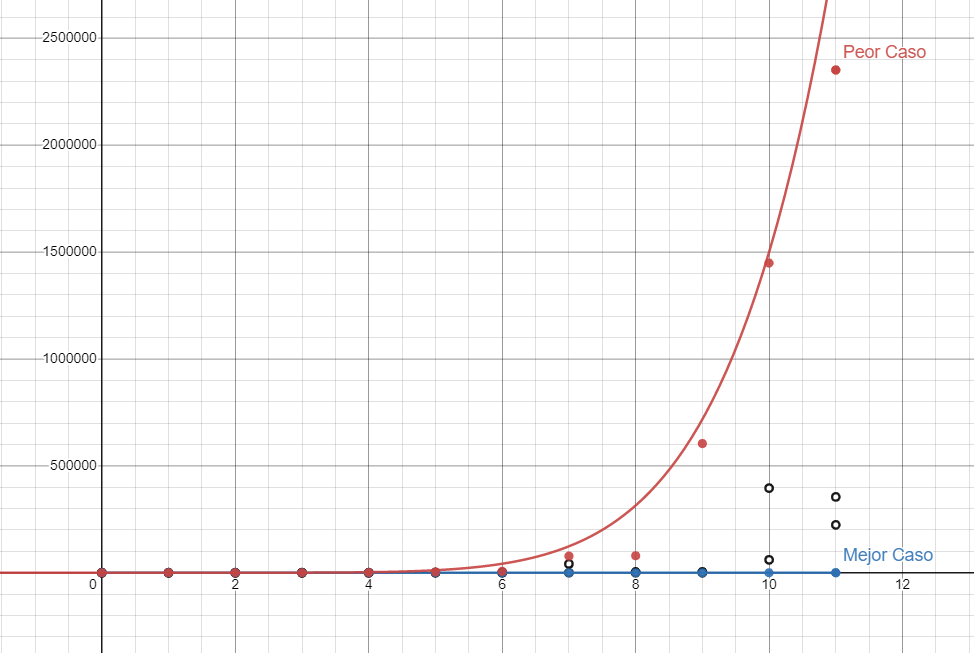
\includegraphics[width=1 \textwidth]{Images/A_Posteriori/posteriori.png}  
            \caption{Análisis a Posteriori: Hamiltoniano}
            \label{fig:posteriori1}
        \end{figure}
    
    
    
    \newpage
    \section{Pantallas de Ejecución del Algoritmo}
    Se muestra en la figura \ref{fig:terminal} la ejecución del algoritmo, demostrando la velocidad del algoritmo.
    
        \begin{figure}[htp!]
            \centering
            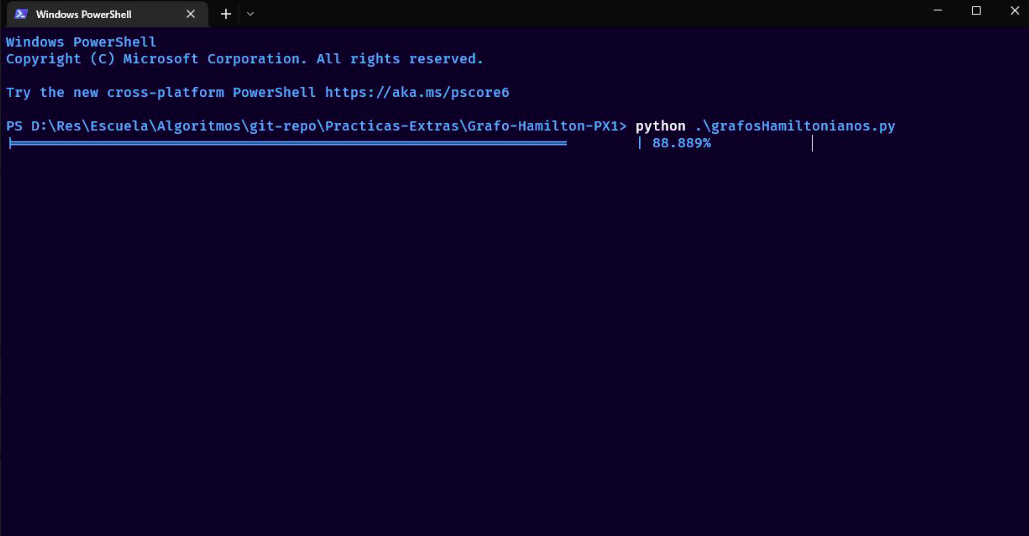
\includegraphics[width=0.8 \textwidth]{Images/Pantallas/PANTALLA.png}  
            \caption{Ejecución de Hamiltoniano}
            \label{fig:terminal}
        \end{figure}
    